%----------------------------------------------------------------------------
\section{Fizika 2}
{\footnotesize Elektromos alapfogalmak és alapjelenségek. Ohm-törvény. A mágneses tér tulajdonságai. Elektromágneses hullámok. A Bohr-féle atommodell. A radioaktív sugárzás alapvető tulajdonságai.}
%----------------------------------------------------------------------------
\subsection{Elektromos alapfogalmak és alapjelenségek.}
\subsubsection{Testek elektromos állapota}
Minden atom magja pozitív töltésű protonokból és töltés nélküli neutronokból áll. A mag körüli elektronhéjon keringenek a protonokkal megegyező számú, negatív töltésű elektronok.\\
Alapesetben az atom kifelé elektromos hatást nem mutat. Ha elektronokat ad le vagy vesz fel, akkor viszont pozitív, illetve negatív töltésű ionná válik. Ennek megfelelően megkülönböztetünk pozitív, negatív és semleges elektromos állapotot.\\
Elektromos szempontból az anyagokat vezetőkre és szigetelőkre oszthatjuk. Az elektromos vezetők mozgásképes töltéshordozókat (elektronokat, ionokat) tartalmaznak. Megkülönböztetünk elsőrendű vezetőket (fémek és a szén), másodrendű vezetőket (elektrolitok és ritkított gázok), félvezetőket, (pl. germánium, szelén, szilícium) amelyek kristályos szerkezetű anyagok és részben vezetők, részben szigetelők. Speciálisak a szupravezetők, amelyek hőmérsékletét csökkentve, a kritikus hőmérséklet elérésekor hirtelen teljesen elvesztik ellenállásukat. Az elektromos szigetelők (pl. üveg, olaj, műanyag) nem tartalmaznak mozgásképes töltéshordozókat.

\subsubsection{Elektromos töltés}
Az anyag alapvető tulajdonsága, bizonyos elemi részecskék jellemzője. Megkülönböztetünk pozitív és negatív töltést. Azonos nemű töltések taszítják, különböző neműek vonzzák egymást.\\
Jele: Q\\
Mértékegysége: Coulomb (C)\\
1 Coulomb = 1As (amperszekundum)\\
Az elektromosan töltött anyag elektromágneses teret hoz létre. Az elektromos töltés kvantált, azaz minden test töltése egy legkisebb töltés többszöröse. Ez a legkisebb töltés az elemi töltés, ami a proton töltése: 1,6 · 10 -19 Coulomb. Az elektron töltése ennek a -1 -szerese. (A kvarkok felfedezése óta úgy gondolják, hogy azok töltése még kisebb lehet, az elemi töltés 1/2, vagy 1/3 része.) Az elektromos töltésre is igaz a megmaradási elv, azaz zárt rendszer töltése állandó. Az elektromos töltések egymásra gyakorolt erőhatásán keresztül a töltés mérhető. A pontszerű töltések között ható (F) erő egyenesen arányos a töltésekkel (Q 1 , Q 2 ) és fordítottan arányos a töltések közötti
távolság (r) négyzetével. Ez Coulomb törvénye.
$$F=k\cdot\frac{Q_1 \cdot Q_2}{r^2}$$
ahol $k$ az arányossági tényező, melynek értéke: $9\cdot10^9 \frac{Nm^2}{C^2}$

\subsubsection{Elektromos Térerősség}
Két pontszerű töltés egymásra gyakorolt hatását úgy is értelmezhetjük, hogy az egyik töltés maga körül elektromos teret hoz létre és ebben a térben a másik töltésre erő hat. Ez az $F$ erő arányos a térben lévő $Q$ töltés nagyságával:
$$F=Q\cdot E$$
Az $E$ arányossági tényező jellemzi az elektromos teret, neve elektromos térerősség. Vektormennyiség, ha a $Q$ töltés pozitív, akkor a töltésre ható erő iránya megegyezik $E$ irányával.
Mértékegysége:$\nicefrac{N}{C}$ és $\nicefrac{V}{m}$

\subsubsection{Fluxus}
Az elektromos mezőt erővonalakkal (Faraday vonalak) szemléltetjük. Az erővonalak bármely pontjába húzott érintő megadja az adott pontban mérhető térerősség irányát, a vonalak sűrűsége pedig a térerősség nagyságával arányos. A fluxus az erővonalak száma. Jele a $\Psi$ (pszi), mértékegysége:$\frac{N}{C}m^2$.
$$ \varPsi = E \cdot A = 4k \cdot \pi \cdot Q $$
$E$ : $Q$ elektromos töltéstől $r$ távolságban a térerősség ($k\frac{Q}{r^2}$)\\
$A$ : egy $r$ sugarú gömb felszíne ($4\pi r^2$)
\begin{theorem}[Gauss-tétel]
	Zárt felületen az elektromos tér fluxusa egyenlő a felületen belül elhelyezkedő töltés $4k\pi$–szeresével. Ha $Q$ pozitív, akkor az erővonalak a felületről kifelé, ha negatív, akkor befelé irányulnak. Tehát minden $Q$ pozitív töltésből $4k\pi Q$ erővonal indul és minden $Q$ negatív töltésben $4k\pi Q$ erővonal végződik.
\end{theorem}

\subsubsection{Elektromos potenciál és feszültség}
Az elektromos mezőbe helyezett töltés az elektromos erő hatására elmozdul, az erőtér munkát végez, a munka nagysága:
$$W = Q \cdot U$$
Ebből a potenciál:
$$U = k\cdot \frac{Q}{r}$$
Az elektromos teret egy kiválasztott pontjához képest fennálló munkavégző képessége szempontjából a potenciál jellemzi. A villamos töltések a villamos tér egyes pontjaiban potenciális energiával rendelkeznek.
Az elektromos tér valamely pontjának potenciálja az a munkamennyiség, amellyel a tér az egységnyi pozitív töltést abból a pontból a nullapotenciálúnak választott pontba képes mozgatni.
Az elektromos tér két pontja közötti feszültség az a munkamennyiség, amellyel a tér az egységnyi pozitív töltést a nagyobb potenciálú pontból a kisebb potenciálú pontba képes mozgatni. A feszültség tehát a két
pont potenciáljának különbsége. 
Így az A és B pont közötti feszültség az A-ból a B-be történő mozgatáshoz szükséges munka és a mozgatott töltés hányadosa:
$$U_{AB} = U_A - U_B = \frac{W_{AB}}{Q}$$
Mértékegysége a Volt. Az elektromos mező két pontja között 1 Volt a feszültség, ha 1 Coulomb töltés átvitelekor az erők 1 Joule munkát végeznek.

\subsubsection{Elektromos áram és áramerősség}
Az elektromos áram a szabadon mozgó töltéshordozók rendezett áramlása. Az elektromos áram létrejöttének feltétele a potenciálkülönbség. Ha az áramlás folyamatosan egyirányú, akkor egyenáramról, ha az áramlás iránya szabályos időközönként megfordul, akkor váltakozóáramról beszélünk.\\
Az áramerősség a vezető keresztmetszetén 1 másodperc alatt átáramló töltések mennyisége:
$$ I = \frac{Q}{t}$$
Mértékegysége az Amper.
1 Ampernyi áramerősség a vezetőréteg keresztmetszetén 1 sec alatt átáramló 1 Coulomb töltést jelent.

\subsubsection{Kapacitás}
Egy rendszer azon képessége, hogy mennyi elektromos töltést képes tárolni. Két vezetőből álló kondenzátor esetén a kapacitás egyenlő az egyik vezetőn felhalmozott töltés és a vezetők közötti feszültség hányadosával:
$$ C = \frac{Q}{U} $$
Mértékegysége a Farad.

\subsubsection{Ohm-törvény}
Egy áramkörben az áramerősség állandó nagyságú ellenállás esetén egyenesen arányos a feszültséggel:
$$U = I \cdot R \quad R = \frac{U}{I}$$
$R$ az ellenállás, ami a vezető anyagi minőségétől, méreteitől és hőmérsékletétől függő állandó.\\
Mértékegysége az Ohm ($\Omega$).\\
1 Ohm ellenállású a vezető, ha abban 1 Volt feszültség 1 Amper erősségű áramot hoz létre.\\
Az ellenállás a vezető hosszával egyenesen, a keresztmetszetével fordítottan arányos:
$$ R = \rho \cdot \frac{1}{A} $$
$\rho$ (ró) a vezető fajlagos ellenállása, ami az anyagi minőségétől és hőmérsékletétől függő állandó.

\subsubsection{Elektromos áram munkája és teljesítménye}
A feszültség: $U = \frac{W}{Q} \rightarrow W = U \cdot Q$\\
Az áramerősség: $I = \frac{Q}{t} \rightarrow Q = I \cdot t$\\
\textbf{Elektromos munkavégzés:} $W = U \cdot I \cdot t$\\
Másképpen: $U = IR,\;I=\frac{U}{R} \rightarrow W = I^2R\cdot t = \frac{U^2}{R} \cdot t$\\
\textbf{Elektromos teljesítmény:}$P=\frac{W}{t}=\frac{UI\cdot t}{t} \rightarrow P=U\cdot I = I^2\cdot R = \frac{U^2}{R}$\\
Az elektromos teljesítmény általános mértékegysége a kilowatt (kW), a munkáé pedig a kilowattóra (kWh).

\subsection{A mágneses tér tulajdonságai. }
Két mágnesrúd egymásra vonzó vagy taszító hatást fejt ki. Az azonos mágneses pólusok taszítják, az ellentétesek vonzzák egymást. Ebből következik, hogy minden mágnes maga körül -- az elektromos erőtérhez hasonlóan -- mágneses erőteret létesít. Az erőteret a térerősséggel, a mágneses indukcióval jellemezhetjük és erővonalakkal szemléltethetjük (\ref{fig:9-eathmagneticfield}~ábra).
\begin{figure}[h]
	\centering
	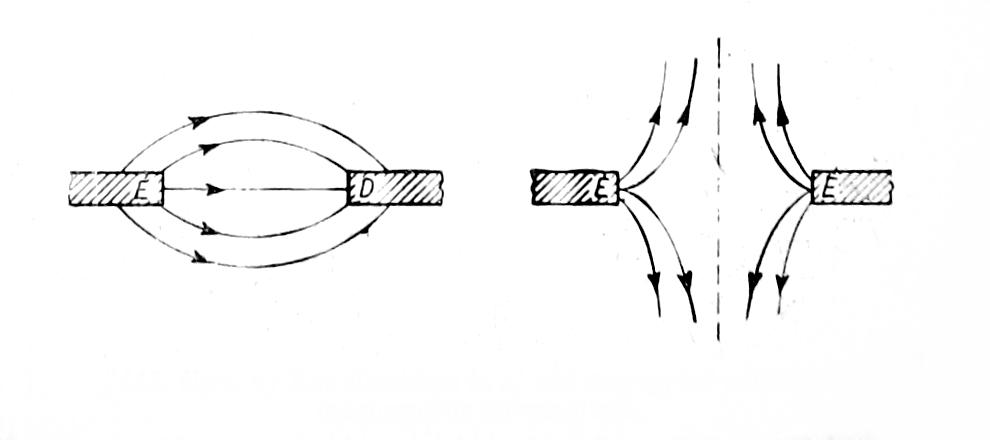
\includegraphics[width=0.7\linewidth]{fig/9-Magnetic_field}
	\caption{}
	\label{fig:9-magneticfield}
\end{figure}

Az erővonalak olyan görbék, amelyek a mágnesben záródnak és irányuk a térben az északi pólustól a déli pólus felé mutat. Ha az erővonalak párhuzamosak és mindenütt egyenlő sűrűségűek, akkor a mágneses tér homogén. A mágneses tér és az elektromos tér legfőbb különbsége, hogy míg az elektromos teret akár a pozitív, akár a negatív töltés egymagában is létrehozza, addig a mágneses teret az északi és déli pólus mindig együttesen létesíti.

Abból, hogy a vízszintes síkban szabadon forgó mágnes mindig észak-déli irányba áll be az következik, hogy a Föld is egy mágnes. A Föld északi sarkán déli, déli sarkán északi mágnesség van. Ezért az erővonalak iránya délről észak felé mutat (lásd:\ref{fig:9-eathmagneticfield}~ábra).
\begin{figure}[h]
	\centering
	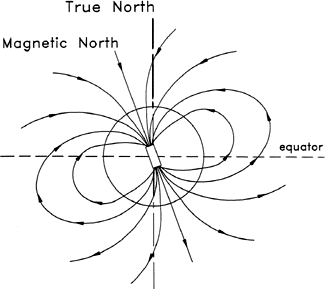
\includegraphics[width=0.3\linewidth]{fig/9-Eath_magnetic_field}
	\caption{}
	\label{fig:9-eathmagneticfield}
\end{figure}

Ha egy vezetőben áram folyik, akkor az mágneses erőteret hoz létre maga körül. A mágneses erővonalak a vezetőre merőleges síkban kialakuló koncentrikus körök, amelyek sűrűsége a vezetőtől távolodva csökken. Az erővonalak irányát jobb kezünk behajlított ujjainak iránya adja, ha hüvelykujjunk az áram irányába mutat. Ha tehát az áram iránya megváltozik, az erővonalak iránya is ellentétessé válik (Jobbkéz-szabály).
\begin{theorem}[Biot--Savart-törvény]
A mágneses térerősség jele $H$. Ha a vezetőben $I$ az áramerősség és $\alpha$ az irányszög, akkor a vezető $\Delta L$ hosszúságú szakasza által, tőle $r$ távolságban létrehozott térerősség nagysága:
$$H=\frac{\mu_0}{4\pi}\cdot\frac{I\cdot \Delta L}{r^2}\cdot \sin \alpha$$
$\mu_0$: permeabilitás
\end{theorem}
A térerősség mértékegysége az Amper/méter.

Egy többmenetes hengeres tekercs mágneses erővonalai az egyes menetek mágneses terének eredőjeként alakulnak ki. Mivel a tekercs belsejében a mágneses tér majdnem homogén, a tekercs egy olyan rúdmágnesnek tekinthető, amelynek hossztengelye egybeesik a tekercs tengelyével (lásd:\ref{fig:9-coil}~ábra).
\begin{figure}[h]
	\centering
	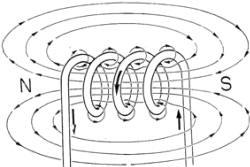
\includegraphics[width=0.3\linewidth]{fig/9-Coil}
	\caption{}
	\label{fig:9-coil}
\end{figure}
Ha egy $N$ menetszámú tekercsben $I$ az áramerősség és a tekercs hossza $L$, akkor a tekercsben a mágneses térerősség:
$$H = \frac{I\cdot N}{L}$$
Ha egy két végén hintaszerűen felfüggesztett vezetőt egy mágnes erőterébe helyezünk és a vezetőn az áramot bekapcsoljuk, akkor a vezető az áram irányára merőleges irányba mozdul ki. Az elmozdulást létesítő $F$ erő nagysága:
$$ F = B \cdot I \cdot L $$
$I$ az áramerősség, $L$ a vezetőnek a mágneses térbe eső hossza, $B$ pedig a mágneses térben lévő anyagtól függő állandó, a mágneses indukció melynek mértékegysége a Tesla.

A mágneses indukciót indukcióvonalakkal jellemezhetjük. Egy adott felületen áthaladó indukcióvonalak száma a mágneses fluxus, ami az indukció és a felület szorzata: $f = B\cdot A$\\
A mágneses fluxus mértékegysége a Weber.

\subsection{Elektromágneses hullámok. }
Az elektromos töltéssel rendelkező testeknek a töltésük miatt fellépő kölcsönhatását az elektromos és mágneses tér segítségével írhatjuk le. A kölcsönhatás úgy működik, hogy egyrészt minden töltés maga körül elektromágneses teret hoz létre, másrészt az elektromágneses tér a töltésekre erőt fejt ki. Így azt mondhatjuk, hogy két töltött test kölcsönhatása az elektromágneses tér közvetítésével valósul meg. Az elektromágneses tér létrehozásához munkát kell végezni, amely munka révén a létrehozott elektromágneses térben energia halmozódik fel. Tudjuk, hogy az elektromágneses tér időbeli változása a térben meghatározott sebességgel (fénysebességgel, amely vákuumban 300 000 km/s) tovaterjed: elektromágneses hullám jön létre, ami energiát visz magával, az elektromágneses tér energiájának sajátos transzportja jön létre. Az elektromágneses hullám energiaszállító képességére utal az elektromágneses sugárzás elnevezés. Egy hozzánk képest nyugvó elektromos töltés elektromos teret, egyenletesen mozgó töltés elektromos és mágneses teret hoz létre maga körül. Kimutatható, hogy a fenti két esetben a tér és a benne felhalmozott energia a töltéstől nem szakítható el, mintegy hozzá van láncolva. Ha azonban a töltés gyorsul, akkor a körülötte kialakuló, időben változó elektromágneses tér elektromágneses hullámot kelt, amely a töltésről leszakadva a térben tovaterjed, és energiát visz magával: a gyorsuló töltés elektromágneses sugárzást bocsát ki magából. Elektromos töltéssel rendelkező testek azonban nemcsak sugározni képesek, hanem a rájuk eső elektromágneses sugárzást el is nyelhetik. Ha ugyanis az anyag egy töltött részecskéjét elektromágneses sugárzás éri, akkor a sugárzás elektromágneses tere a tér által a töltésre ható erő révén a részecskét felgyorsítja, miáltal a test a ráeső sugárzás egy részét elnyeli. A fenti két folyamat teszi lehetővé, hogy két test kölcsönhatásba léphet egymással úgy is, hogy az egyik a másiknak elektromágneses sugárzás formájában energiát ad át. Ennek a jelenségnek számos konkrét példáját ismerjük. Az elektromágneses sugárzás útján történő energiaátadás közismert példája az elektromágneses hullámokkal megvalósított távközlés (rádió, TV): egy rádióadóban pl. a továbbítandó elektromos jellel (váltakozó áram) rezgőmozgásba (gyorsuló mozgás) hozzák az adóantenna elektronjait, amelyek ennek megfelelő elektromágneses sugárzást bocsátanak ki. Ennek a sugárzásnak egy része eléri a vevőkészülék antennáját, és a benne lévő elektronokat a sugárzás elektromos tere rezgésbe hozza. Az elektronoknak ez a rezgőmozgása (váltakozó áram) azután a vevőkészülékben létrehozza a leadott jelnek megfelelő elektromos jelet. A sugárzásos energiaátadás másik, közismert példája a hőmérsékleti sugárzás kibocsátása és elnyelése. Tapasztalati tény, hogy az anyagok a hőmérsékletüktől függően különböző hullámhosszú elektromágneses sugárzást bocsátanak ki magukból, s a rájuk eső sugárzás egy részét elnyelik.

A foton az elektromágneses hullámok elemi részecskéje. A fotonok nyugalmi tömege nulla, sebességük a fénysebesség. Az elektromágneses hullám keletkezése atomi szinten úgy történik, hogy a gerjesztés hatására az atommag körül keringő elektron egy nagyobb energiájú pályára ugrik, majd onnan eredeti pályájára visszazuhanva egy fotont bocsát ki. A keletkező foton hullámhossza az energiaszintek különbségétől függ.

A különböző körülmények között létrejött elektromágneses sugárzások lényegében a kibocsátott hullám hullámhosszában és ezzel együtt frekvenciájában térnek el egymástól, és ez eredményezi azt, hogy az anyaggal való kölcsönhatásaik, az anyagra gyakorolt hatásaik is eltérőek.Az elektromágneses sugárzás hullámhossz szerinti felosztása, az ún. elektromágneses spektrum (lásd:\ref{fig:9-electromagneticspectrum}~ábra)
\begin{figure}[h]
	\centering
	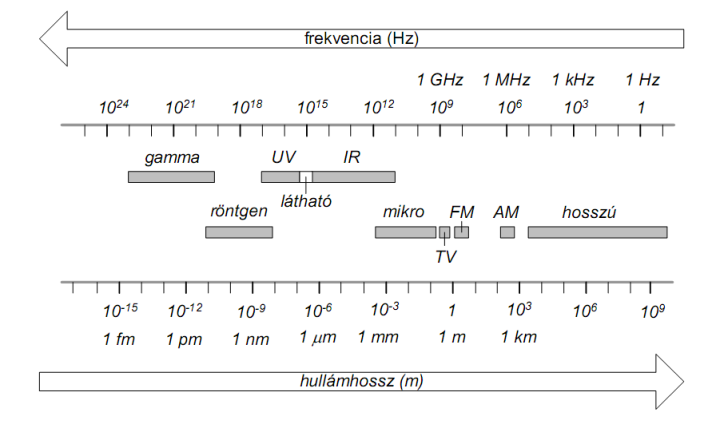
\includegraphics[width=0.7\linewidth]{fig/9-Electromagnetic_spectrum}
	\caption{}
	\label{fig:9-electromagneticspectrum}
\end{figure}

A fény szűkebb értelemben az elektromágneses spektrumnak az a része, amelyet az emberi szem érzékelni képes (kb. 350-től 750 nanométerig). Tágabb értelemben ide sorolják a tartományhoz közvetlenül csatlakozó hosszabb hullámhosszú infravörös- és a rövidebb hullámhosszú ultraibolya sugárzást is. Az emberi szem érdekes sajátsága, hogy a különböző hullámhosszú fényt különböző színűnek észleli. A klasszikus felfogás szerint a fényhullámként terjed, tehát érvényesek rá mindazok az általános törvények, amelyek a hullámokra érvényesek. A fénynek azonban vannak, elektromágneses jellegével és a hullámhosszával összefüggő, speciális tulajdonságai is.

A fény egy anyagban terjedve, és egy határfelülethez érve részben behatol az új anyagba, részben pedig visszaverődik a határfelületről. Vannak anyagok, amelyekbe a fény gyakorlatilag nem tud behatolni, mert a határfelületeikről a fénysugárzás nagyobb része visszaverődik, vagy igen rövid távolságon belül elnyelődik. Az anyagok egy része a fényt többé-kevésbé átereszti, ezeket az anyagokat legtöbbször átlátszó anyagoknak nevezzük. A fény és anyag kölcsönhatása általában függ a fény hullámhosszától, így egy anyag bizonyos hullámhosszakra lehet áteresztő, más hullámhosszakat viszont elnyel.

Az elektromágneses hullámok létezését elméletben Maxwell (1864), kísérletileg Hertz mutatta ki (1888).

\subsection{A Bohr-féle atommodell.}
Az 1900-as évek elején Ernest Rutherford megalkotta róla elnevezett atommodelljét, amely szerint az atom középpontjában van a pozitív töltésű atommag, ami körül keringenek az elektronok. Az atom kifelé semleges, tehát az elektronok száma egyenlő az atommag pozitív töltésének a számával. A modell legnagyobb hibája az volt, hogy mivel a keringő elektronok váltakozó elektromágneses teret hoznak létre maguk körül, ezzel együtt energiát kell kisugározniuk, viszont az energia kisugárzás csökkenti az elektron mozgási energiáját, így az elektron egy idő után az atommagba kellene, hogy essen.

1913-ban Niels Bohr dán fizikus a Rutherford-féle atommodell módosításával megalkotta saját atommodelljét, amely szerint:
\begin{enumerate}[nosep]
	\item Az atom normális (gerjesztés nélküli) állapotában az elektron csak meghatározott pályán keringhet és 	ebben az esetben nem sugároz energiát. Emellett azt is feltételezte, hogy az elektronpályák sugarai úgy aránylanak egymáshoz, mint a természetes egész számok négyzetei:
	\begin{figure}[h]
		\centering
		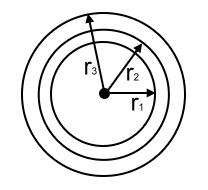
\includegraphics[width=0.25\linewidth]{fig/9-Atom_eletrontracks}
		\caption{$r_1 : r_2 : r_3 = 1 : 4 : 9$}
		\label{fig:9-atomeletrontracks}
	\end{figure}
	
	\item A megengedett pályákon keringő elektronoknak meghatározott energiájuk van, amelyet mozgási energiájuk és az elektromos erőtér potenciális energiája határoz meg. Egy elektron összenergiája a nagyobb sugarú pályán nagyobb.
	\item Ha az atommal energiát közlünk, akkor az elektron átugrik egy másik, nagyobb sugarú pályára. Ez az ún. gerjesztés. A gerjesztéskor felvett energia megegyezik a két pályához tartozó energiaértékek különbségével. A gerjesztett atom azonban instabil, így az elektron a nagyobb energiájú pályáról a maghoz közelebbi kisebb energiájú belső pályára ugrik és az energiakülönbséget elektromágneses hullám formájában kisugározza.
\end{enumerate}

\subsection{A radioaktív sugárzás alapvető tulajdonságai.}
Becquerel francia fizikus 1896-ban kutatásai során megállapította, hogy az uránszurokérc olyan sugarakat bocsát ki magából, amelyeknek nagy az áthatolóképességük, a levegőt ionizálják. Két évvel később a Curie házaspárnak sikerült az uránércből az uránnál kb. milliószor erősebben sugárzó anyagot a rádiumot kiválasztani. Később még ennél is erősebben sugárzó anyagot találtak, ez a polónium. A további kutatások során megállapították, hogy ilyen radioaktív sugarakat még sok más elem is kibocsát és ezekre az anyagokra jellemző, hogy külső behatás nélkül, állandóan sugároznak.

A radioaktív sugárzás a radioaktív bomlás során keletkezik. A bomlás izotópokban megy végbe. Majdnem valamennyi a természetben előforduló elem izotópok keverékéből áll. Egy elem izotópjai, az elemmel azonos rendszámú, de eltérő tömegszámú és atomsúlyú elemek. Egy adott elem mindegyik izotópja ugyanannyi protont és elektront, de eltérő számú neutront tartalmaz. Egy elem izotópjai kémiailag teljesen azonosak, de fizikai tulajdonságaik eltérnek. Azokat, amelyeknél nem figyeltek meg radioaktív bomlást, stabil izotópoknak nevezik, míg, amelyeknél megfigyeltek azok instabil izotópok. Egy elem csak meghatározott proton/neutron arány esetén stabil. Nagyon sok elemnek vannak természetes radioaktív izotópjai. Vannak olyan elemek, amelyeknek csak radioaktív izotópja létezik (pl. polónium, radon, rádium), viszont mesterségesen minden elemnek előállítható radioaktív izotópja.

A radioaktív bomlás során a radioaktív izotópok instabil atomjai hosszabb-rövidebb idő elteltével alacsonyabb energiaszintű állapotba mennek át, és eközben emberi érzékszervekkel nem észlelhető, de műszerekkel jól kimutatható radioaktív sugárzást bocsátanak ki.

A bomlás mértéke lemérhető. Az 1 másodperc alatt bekövetkező bomlások száma az aktivitás. Mértékegysége a Becquerel. 1 Bq = 1 bomlás/másodperc.

A bomlást a felezési idővel is jellemezhetjük, ez az az idő, amely alatt egy bizonyos mennyiségű anyag atomjainak a száma radioaktív bomlással a felére csökken. Másodpercektől éves nagyságrendekig változhat, akár sok millió vagy milliárd év is lehet.

A bomlás során keletkező sugárzásnak 3 fajtáját különböztetjük meg:
\begin{description}
	\item[Alfa-sugárzás] Pozitív töltésű héliumionokból áll. Töltésük az elemi töltés kétszerese, tömegük kb. a hidrogénatom tömegének négyszerese, sebességük függ a kibocsátó anyagtól. Az alfa-sugaraknak nagy az áthatolóképességük és erősen ionizálnak, viszont a levegőmolekulákkal való ütközés során hamar lefékeződnek, így hatótávolságuk kevesebb, mint egy centiméter.
	\item[Béta-sugárzás] elektronok vagy pozitronok (béta-részecskék) alkotják. Sebességük széles skálán változik, de jóval nagyobb, mint az alfa-sugárzás esetében és bár tömegük jóval kisebb, mint az alfa-részecskék tömege, a nagy sebesség miatt hatótávolságuk levegőben néhányszor tíz centiméter.
	\item[Gamma-sugárzás] agy energiájú elektromágneses sugarak, frekvenciájuk elérheti a 10\textsuperscript{21} Hz értéket. Hatótávolságuk végtelen, a nagy tömegszámú és sűrűségű elemek (pl. ólom) viszont hatékonyan gyengítik.
\end{description}
A bomlásokat az általuk létrehozott sugárzás alapján különböztetjük meg. Eszerint van alfa-, béta- és gamma-bomlás.